\documentclass{article}
\usepackage[utf8]{inputenc}
\usepackage{amsmath}
\usepackage{natbib}
\usepackage{graphicx}

\begin{document}
\section*{Blatt 1 - Cerberus}
\subsection*{Aufgabe 2}
Für den Datensatz
\begin{table}
    \centering
\label{tab:data_tab}
	\sisetup{table-format=1.2}
	\begin{tabular}{S[table-format=2.1]S[table-format=2.1]}
		\toprule
		{$x$} & {$y$} \\
		\midrule
		0.0 & 4.0 \\
		2.5 & 4.3 \\
		-6.3 & -3.9 \\
		4.0 & 6.5 \\
		-3.2 & 0.7 \\
		5.3 & 8.6 \\
		10.1 & 13.0 \\
		9.5 & 9.9 \\
		-5.4 & -3.6 \\
		12.7 & 15.1 \\
		\bottomrule
	\end{tabular}

\end{table}
soll eine lineare Regression der Form
\[
y = mx + n
\]
durchgeführt werden, die den quadratischen Fehler minimiert.\\
Zunächst lässt sich das lineare Gleichungssystem $A\vec{x}=\vec{b}$ aufstellen als
\[
\begin{pmatrix}
   0  & 1\\
 2.5  & 1\\
-6.3  & 1\\
   4  & 1\\ 
-3.2  & 1\\
 5.3  & 1\\
10.1  & 1\\
 9.5  & 1\\
-5.4  & 1\\
12.7  & 1
\end{pmatrix}\cdot
\begin{pmatrix}
m\\
n
\end{pmatrix} = 
\begin{pmatrix}
4\\
4.3\\
-3.9\\
6.5\\
0.7\\
8.6\\
13\\
9.9\\
-3.6\\
15.1
\end{pmatrix}
\]
Durch multiplizieren mit der Transponierten der Matrix $A$ wird wandelt sich das
System zu $A^TA\vec{x} = A^T \vec{b} = \vec{b}'$, mit der quadratischen Matrix
\[
A^TA = \begin{pmatrix}
482.98 & 29.2 \\
  29.2  &  10 
\end{pmatrix}
\]
und dem neuen Ergebnisvektor
\[
\vec{b}' = \begin{pmatrix}
541.22\\
  54.6
\end{pmatrix}\text{.}
\]
Eine numerische LU-Zerlegung $A^TA = PLU$ liefert die Pivotisierungs-Matrix
\[
P = 
\begin{pmatrix}
1 & 0\\
0 & 1
\end{pmatrix},
\]
die L-Matrix
\[
L = \begin{pmatrix}
       1    &   0\\
0.060458    &   1
\end{pmatrix}
\]
und die U-Matrix
\[
U = \begin{pmatrix}
 482.98 &  29.2\\
      0 & 8.23463
\end{pmatrix}.
\]
Damit ergibt sich die Lösung für die lineare Regression zu
\[
y = 0.959951\cdot x + 2.65694\; .
\]
In Abbildung \ref{fig:linreg} ist diese Ausgleichsgerade und die zugehörigen Daten zu sehen.
\begin{figure}
    \centering
    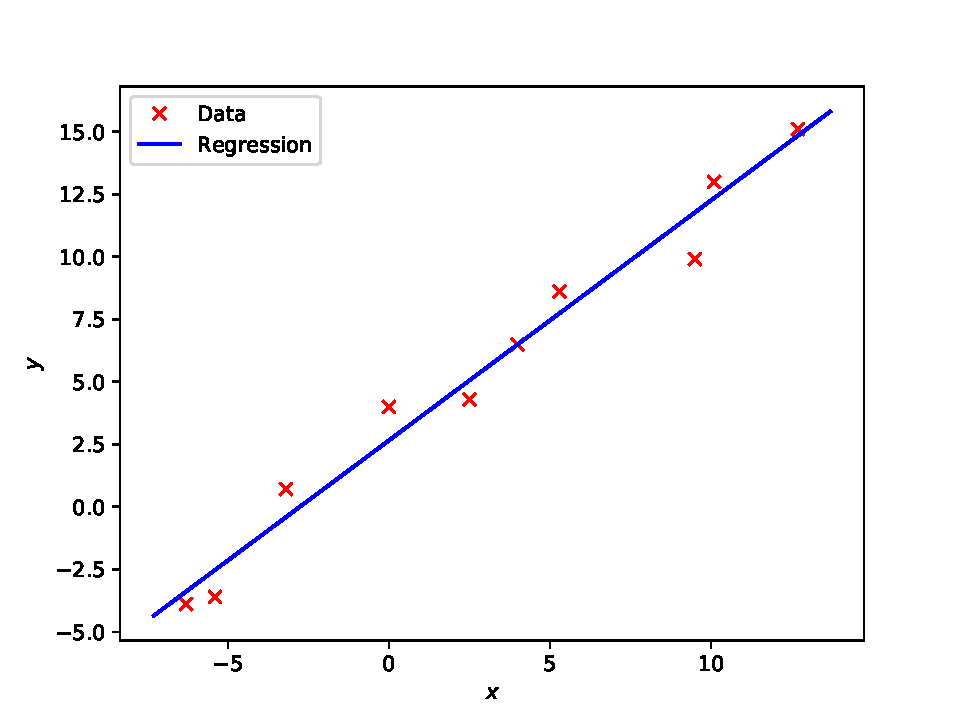
\includegraphics[width=\textwidth]{A2/build/Regression.pdf}
    \caption{Lineare Regression zum Datensatz\ref{tab:data_tab}.}
    \label{fig:my_label}
\end{figure}

\end{document}
